% !TeX spellcheck = en_GB
\chapter{Analysis}
\epigraph{Without requirements or design, programming is the art\\of adding bugs to an empty text file.}{Louis Srygley}
\section{Terminology}
Taking into account that developers and operators of security reporting systems are the intended audience for this thesis,
we mostly use the  Security Automation and Continuous Monitoring (SACM) terminology~\cite{ietf-sacm-terminology-14}
and thereby follow the same guidelines as the \gls{xmpp-grid-standard}~\cite{ietf-mile-xmpp-grid-05}.

\section{Technical Background}\label{sec:technical-background}

The following sections introduce the \gls{xmpp} protocol including its terminology and summarise the relevant extensions (\glspl{xep}) used by the \gls{xmpp-grid-standard}.

\subsection{XMPP (Extensible Messaging and Presence Protocol)}
The Extensible Messaging and Presence Protocol (in short \gls{xmpp}, formerly known as \gls{jabber}) is an open protocol that enables the near-real-time exchange of small data between any network endpoints, hereafter called \glspl{platform}~\cite{rfc6120}.
While originally designed as an instant messaging (IM) protocol, \gls{xmpp} can be used for a wide range of data exchange applications~\cite{ieee-xplore-stream-xml-xmpp}.

\gls{xmpp} is made of small building blocks defined in the core protocol~\cite{rfc6120} and numerous extensions called \glspl{xep}~\cite{xep-0001}.
The core specifies how encrypted communication channels must be established, how \gls{xml} \glspl{stanza} are exchanged and errors are handled.

The core is comprised of \gls{xml} streams, error handling and functionality for establishing encrypted communication channels.
Additional functionality such as \gls{service-discovery}~\cite{xep-0030} and \gls{publish-subscribe}~\cite{xep-0060} are defined in separate extensions.

Although \gls{xmpp} supports peer-to-peer communication, it is often used in a traditional client-server architecture.
A client (\gls{platform}) can send data to any addressable entity (any other \glspl{platform}) using \Gls{jabber} identifiers, hereafter called \gls{jid}.
If the receiving \gls{jid} has a different domain than the current server (\gls{controller}), the message is forwarded to the \gls{xmpp} server responsible for this domain.~\cite{rfc6120}

The data exchanged over \gls{xmpp} is in the \gls{xml} format, which makes the protocol structured and extensible, but leads to some protocol overhead.
An \gls{xmpp} client communicates with the server over unidirectional data streams, that are basically long-lived \gls{tcp} connections.
A client opens a channel to the server over this connection, and the server reacts by opening a connection in the opposite direction.
In both streams, an XML document is opened after the connection is established (i.e. with \code{<stream>} XML tags).
During the conversation, an arbitrary amount of \glspl{stanza} (specified XML child elements) are written to the stream.
Before a connection may be terminated, the root element is closed (i.e. \code{</stream>}) and both streams form valid XML documents~\cite{rfc6120}\cite{professional-xmpp}.

The core \gls{stanza} types are \glspl{message}~(\code{<message/>}), \gls{presence}~(\code{<presence/>}) and\\
\gls{info-query}~(\code{<iq/>}).
\Glspl{message} can contain arbitrary data similar to email but are optimised for immediate delivery.
\Gls{presence} \glspl{stanza} deal with network availability and the propagation of user presence information.
An \gls{info-query} \gls{stanza} consists of a request and response (similar to the GET and POST HTTP methods), which is used for feature negotiation, configuration and general information exchange.
Because of these coarse semantics, \gls{xmpp} provides a generalized communication layer~\cite{rfc6120}\cite{ieee-xplore-stream-xml-xmpp}.

Figure~\ref{fig:xmpp-overview} illustrates an example setup with two servers and three clients.

\begin{figure}[h]
	\centering
	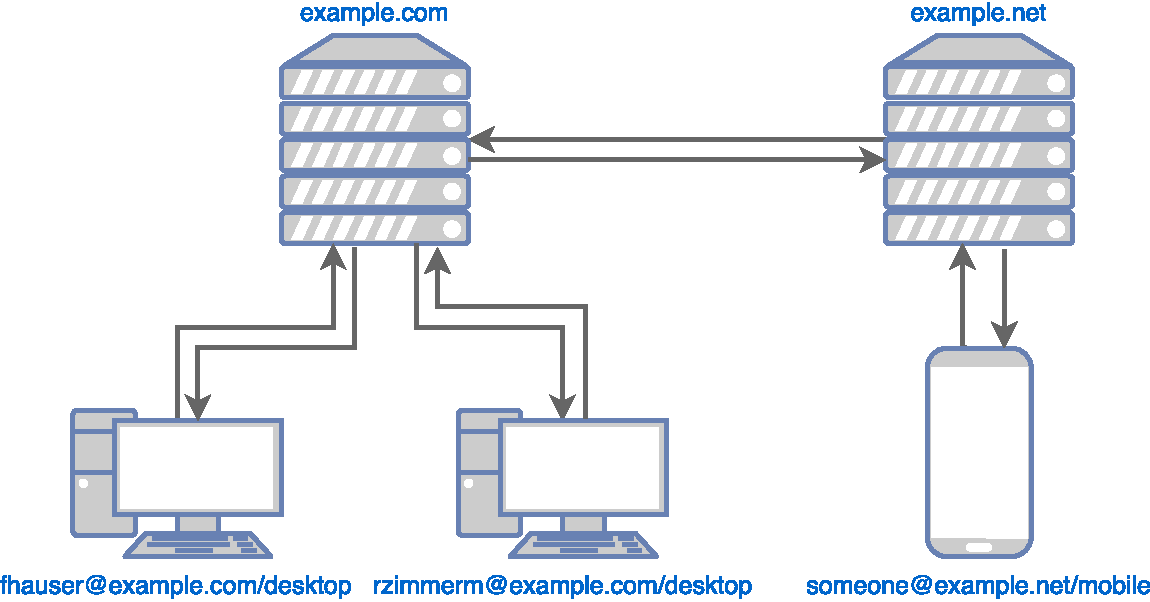
\includegraphics[width=0.8\linewidth]{resources/xmpp_overview.pdf}
	\caption[XMPP example overview]{Two \gls{xmpp} domains (servers), one with two users and one with a single mobile user.}
	\label{fig:xmpp-overview}
\end{figure}

\subsection{Relevant XMPP Extensions}

The \gls{xmpp-grid-standard} is based on multiple \glspl{xep}, most notably the \gls{publish-subscribe} extension. In this section, we give an overview of the most relevant used \glspl{xep}.

\paragraph{XEP-0004: Data Forms} is a flexible protocol that can be used in workflows such as service configuration.
The protocol provides form processing, common field types and extensibility mechanisms.~\cite{xep-0004}

\paragraph{XEP-0030: Service Discovery} enables entities to discover information about the identity and capabilities of other entities, e.g. whether the entity is a server or not, or items associated with an entity, e.g. a list of \gls{publish-subscribe} nodes.~\cite{xep-0030}

\paragraph{XEP-0059: Result Set Management} allows entities to manage the receipt of large result sets, e.g. by paging through the result or limiting the number of results. \gls{result-set-management} is often desired when dealing with large dynamic result sets, as from service discovery or publish-subscribe, and when time or other resources are limited.~\cite{xep-0059}

\subsubsection{XEP-0060: Publish-Subscribe}
The \gls{publish-subscribe} extension, hereafter referred to as \gls{pubsub} or \gls{broker}, enables \gls{xmpp} entities (\glspl{provider}) to broadcast information via \glspl{topic} to subscribed entities (\glspl{consumer}).~\cite{xep-0060}

Nodes, hereafter referred to as \glspl{topic}, are the communication hubs. Entities can create \glspl{topic} and configure them, e.g. set up subscription timeouts or limit publishing and subscription rights. The configuration mechanism is based on data forms (XEP\babelhyphen{nobreak}0004).
An \gls{xmpp} server \emph{may} restrict \gls{topic} creation to certain entities, which means that possibly not every \gls{xmpp}-Server that supports \gls{publish-subscribe} also implements this feature \cite{rfc2119}.

The protocol defines a hierarchy of six affiliations of which only the implementation of owner and none is \emph{required}.
Implementing the remaining four affiliations is \emph{recommended}.
An owner of a \gls{topic} can manage the subscriptions and affiliations of other entities associated with a given \gls{topic}.

To simplify the creation of \glspl{topic}, \gls{pubsub} defines five \gls{topic} access models (node access models) that \emph{should} be available: open, presence, roaster, authorize and whitelist.
The open model allows uncontrolled access while presence and roaster are specific for IM. Using the authorize model, the owner has to approve all subscription requests.
The whitelist model enables the owner to maintain a list of entities that are allowed to subscribe.


\section{Domain Analysis}

\subsection{IETF Standard Draft: Using XMPP for Security Information Exchange}\label{sec:ietf-standard-draft-using-xmpp-for-security-information-exchange}
This \gls{ietf} standard draft describes how the \gls{xmpp} protocol and its extensions can be used for the exchange and distribution of security-relevant information between network devices.

One of the primary motivation for using \gls{xmpp} for this task is the fast propagation of such security-relevant data.
Using \gls{xmpp} for such a task also comes with its downsides. Most notably, because the \gls{xmpp} server (\gls{broker}/\gls{controller}) is the central configuration component in charge of managing access permission, its compromisation has serious consequences.

The standard describes a trust model, a thread model as well as specific countermeasures, e.g. to use at least \gls{tls} 1.2. These countermeasures also define restrictions of the \gls{xmpp} protocol and its extensions, e.g. by limiting the \gls{topic} access models of \gls{pubsub} to whitelist and authorized only~\cite{ietf-mile-xmpp-grid-05}.

\subsubsection{Information Exchange Format}

The \gls{xmpp-grid-standard} states that `although [the exchanged] information can take the form of any structured data (XML, JSON, etc.), this document illustrates the principles of \gls{xmpp-grid} with examples that use the Incident Object Description Exchange Format (IODEF)'~\cite{rfc7970, ietf-mile-xmpp-grid-05}.

As IODEF is not strictly defined nor explicitly recommended by the \gls{xmpp-grid-standard}, no specific integrations are in the scope of this thesis.

In practice, small payloads are sent over an \gls{xmpp-grid}, usually containing external pointers to an API that provides more comprehensive data (see appendix~\fullref{sec:meeting-minutes}).

\subsection{Domain Specific Language}

Figures~\ref{fig:architecturedslgriddraft} and \ref{fig:architecturedslxeps} present an overview of the relevant interactions and relationships between the different components as specified in the \gls{xmpp-grid-standard} and the referenced \glspl{xep} (see Section~\fullref{sec:technical-background}).

\begin{figure}[h]
\centering
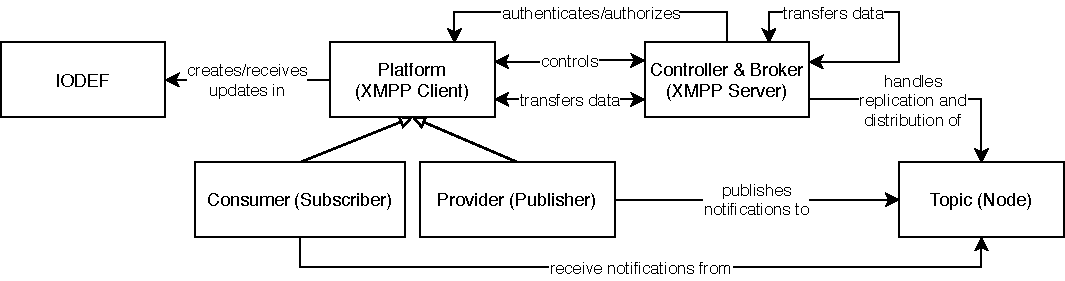
\includegraphics[width=\linewidth]{resources/architecture_dsl_grid_draft}
\caption[DSL of the XMPP-Grid standard]{Domain specific language of the \gls{xmpp-grid-standard}.}
\label{fig:architecturedslgriddraft}
\end{figure}

\begin{figure}[h]
\centering
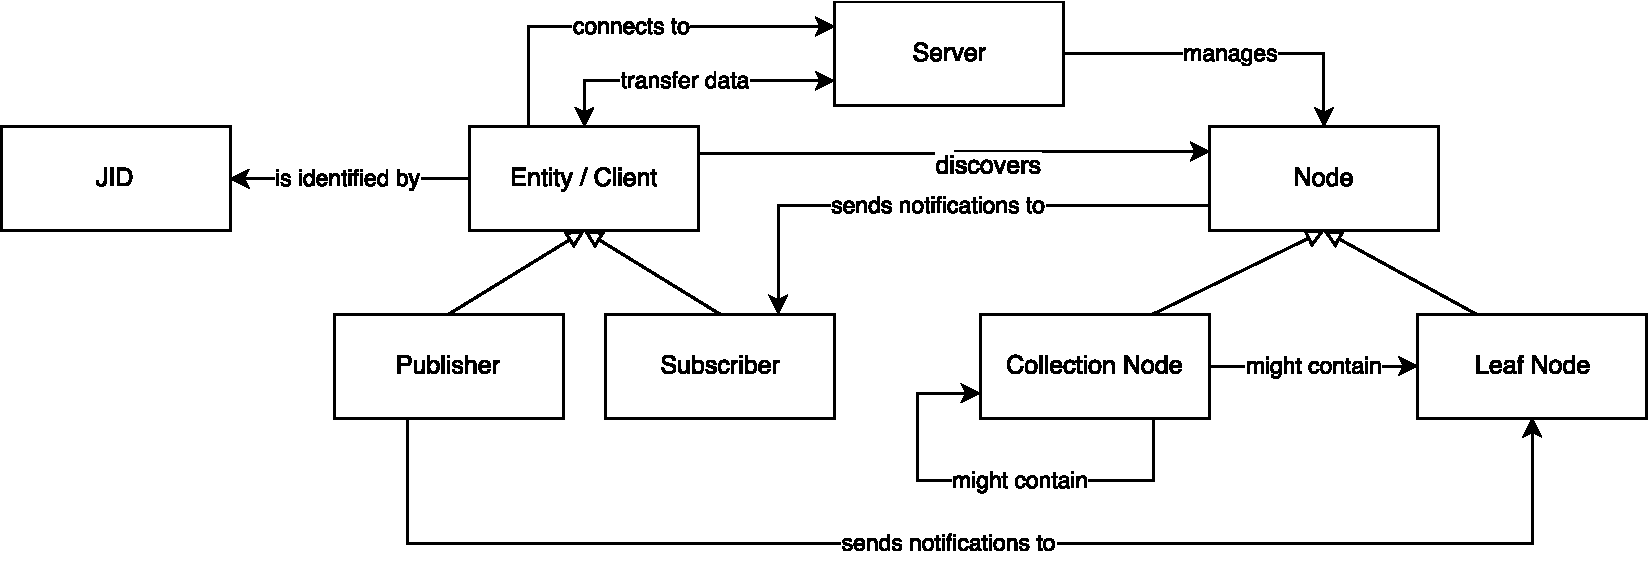
\includegraphics[width=\linewidth]{resources/architecture_dsl_xeps}
\caption[DSL of used XMPP XEPs]{Domain specific language of used \gls{xmpp} \glspl{xep}.}
\label{fig:architecturedslxeps}
\end{figure}

\section{Requirements Analysis}

We collected the functional requirements in the form of user stories.
User stories are an established and widespread concept for describing and managing requirements in agile software projects.
In comparison to traditional tools for requirement analysis, user stories are more concise, leaving more space for change. \cite{wirdemann2017scrum}

We also created user stories for non-functional requirements.
Additional non-functional requirements can be added during the project in the form of constraints. \cite{wirdemann2017scrum}

In the early phase of the project, we collected an initial set of user stories in collaboration with Prof.\ Dr.\ Steffen.
This initial set covered the creation and deletion of \glspl{topic} as well as  granting publish and subscribe privileges.
All user stories are listed in Appendix~\fullref{sec:requirements}.

After setting broad priorities, Prof.\ Dr.\ Steffen approved the initial set of user stories that then served as the basis for the architectural concept.